\documentclass{subfiles}
\begin{document}
\section{Intermediate results of system and basis study}\label{sec:general_study_results}
We here present the results of our study of the Morse double-well potential, and the validity of the Sinc-DVR basis for the system. First the analysis showcasing how the exchange term is negligible in th double-well system is presented, followed by a validation of the Sinc-DVR basis against the exact analytical eigenstates in a single-well system. Finally, we present a benchmark of the numerical methods used for time-evolution, using the Landau-Zener model as a testbed. This section serves as an intermediate step towards the final results presented in later sections.

\subsection{Exchange interaction in the Morse double-well}\label{sec:exchange_interaction}
In our Hartree product-state approach (Section \ref{sec:Hartree_method}), we include only the direct Coulomb interaction between the particles. This explicitly neglects exchange effects, justified by our intent to construct a system with strictly localized—and thus distinguishable—particles. Although exchange cannot create entanglement, it can influence energy spectra by shifting single-particle levels and modifying the composition of the reduced Hartree basis. To rigorously test our approximation, we benchmark our Hartree results against a fully antisymmetrized calculation performed using the configuration-interaction (CI) method described in detail in Section \ref{sec:CI_method}, following the procedure outlined in Section \ref{sec:distinguishability}.

Recall that in the Hartree product-state approach, the two-particle Hamiltonian is given by
\begin{align*}
    H_{dist} = H_L \otimes \mathbb{I} + \mathbb{I} \otimes H_R + V_{LR},
\end{align*}
where $H_L$ and $H_R$ are the single-particle Hamiltonians of the left and right wells, respectively, and $V_{LR}$ is the direct Coulomb interaction between the particles—and the Hartree energies are found by direct diagonalization of this Hamiltonian. In the CI approach, we start from the same two-particle Hamiltonian but build a projection onto the anti-symmetric subspace spanned by all unordered pairs of single-particle states. 

We carry out both calculations, Hartree and CI diagonalization as a function of inter-well separation $d$. In both solvers, we use a Sinc-DVR basis with $N=800$ gridpoints and  grid length of $L=400$ a.u. This yields a grid spacing of $\Delta x = 0.5$ a.u. and a grid wide enough to encapsulate the system equally for all inter-well separations considered in the analysis. The grid spacing is chosen to be small enough to ensure convergence of the results. For CI we build the $N$ lowest single-particle orbitals and retain $\binom{N}{2}$ anti-symmetric states. We define the exchange-induced shift
\begin{align*}
    \Delta E = E_{CI} - E_{Hartree},
\end{align*}
where $E_{CI}$ is the ground-state energy obtained from the CI diagonalization and $E_{Hartree}$ is the ground-state energy obtained from the Hartree product state approach. The exchange shift $\Delta E$, as discussed in Section \ref{sec:distinguishability}, quantifies the exchange interaction energy contribution, and is visualized alongside the two ground-state energies in figure \ref{fig:exchange_shift}. As the wells move farther apart, the exchange interaction energy falls off sharply, dropping below the numerical noise floor for separations $d > 10$ a.u, which is 10 $a_0$. Following the discussions in Appendix \ref{app:appendix_A}, this corresponds to an effective inter-well separation of approximately $100$ nm in a GaAs quantum dot system, well within the working ranges for quantum dots \cite{jacak2013quantum, garcia2021semiconductor}.

\begin{figure}[h!]
    \centering
    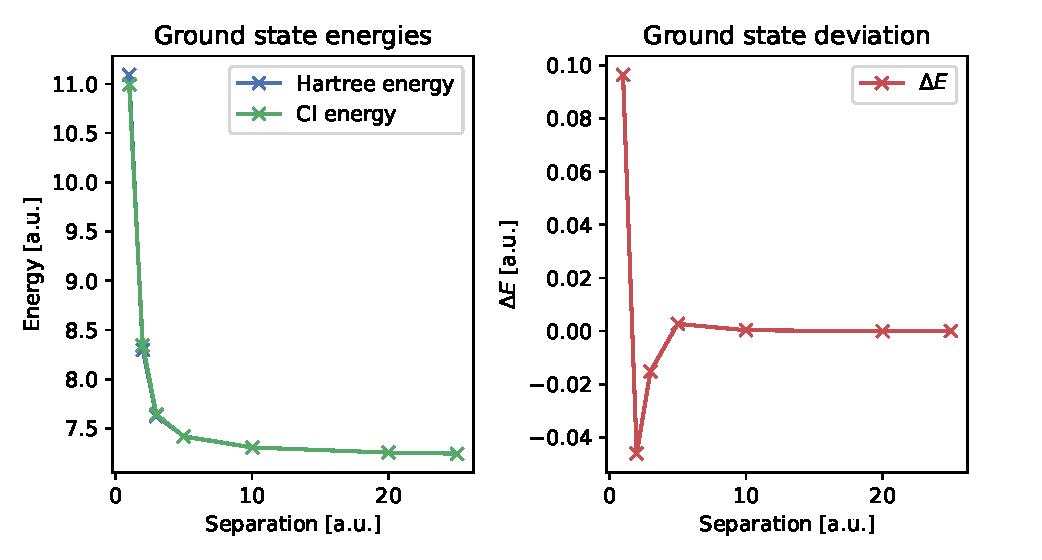
\includegraphics[width=1.0\textwidth]{figs/exchange_shift.pdf}
    \caption{Ground-state energy as a function of the inter-well separation $d$ for the Morse double-well potential for Hartree (blue) and CI (green). The rapid decay of the exchange term of the coulomb interaction matrix with increasing well separation indicates that this term has a negligible effect on the ground state energy, confirming our assumption of locality and the usage of product states to express the wavefunction, as the particles become distinguishable for appropriate separation. We can see that the exchange term is close to zero for well separations larger than $d = 10$a.u., since $\Delta E=0$. We also see the non-variational nature of the Hartree product state, as for some separations, the Hartree energy estimate falls below that of truncated CI, seen as a negative $\Delta E$.}
    \label{fig:exchange_shift}
\end{figure}
We observe in figure \ref{fig:exchange_shift} that the exchange interaction has a near-zero contribution beyond moderate separations, confirming that exchange contributions are truly negligible for our system—and that the Hartree product state captures the correct low-energy physics. This vindicates our assumption that the particles are distinguishable: once the two wells are sufficiently separated, the Pauli exclusion principle has vanishing impact of both energies and wavefunctions. The parameters used for this simulation are the optimal parameters for the Morse double-well configuration $C_I$ \ref{tab:optimized_params}, as described in section \ref{sec:optimization_procedure} and presented in Section \ref{sec:optimization_result}. 

A final caveat: because the Hartree product state is not anti-symmetric, the Hartree energy is not variational with respect to exchange (it can lie slightly below the true anti-symmetric energy in a truncated basis, as seen in figure \ref{fig:exchange_shift}). One must therefore thread carefully when interpreting the energies obtained from the Hartree product state. In our tests, however, we find no (strictly) un-physical energies—the Hartree energy is within sub meV of the CI energy for all separations considered. We therefore conclude that for all practical purposes, the product state Hartree approximation suffices and this justifies neglecting exchange in our time-evolution simulations.


\subsection{Sinc-DVR basis validation}
\subsubsection*{Energy eigenstates}
A natural validation of the Sinc-DVR basis is to check that the Sinc-DVR basis functions closely match the exact energy eigenstates of the system. We require that the eigenfunctions built from the Sinc-DVR basis to have a high degree of overlap with the exact energy eigenstates of the system. Otherwise, we risk losing important information about dynamics of the system, dynamics that may have a significant impact on the quantum control protocols we wish to implement.\\ 

We begin by computing the overlap matrix $S$ between the Sinc-DVR basis functions and the exact energy eigenstates of the Morse potential, from the analytical expressions in Section \ref{sec:basis_set}. Recall, the overlap matrix is defined as:
\begin{align*}
    S_{ij} = \int \psi_i(x) \psi_j(x) dx,
\end{align*}
where $\psi_i(x)$ and $\psi_j(x)$ are the Sinc-DVR basis and exact energy eigenstates, respectively using the procedures outline in Section \ref{sec:sinc_dvr_validation}.

The overlap matrix $S$ is then a measure of how well the Sinc-DVR basis functions represent the exact energy eigenstates of the system. The results are shown in figure \ref{fig:dvr_validation_overlap}, where we see that the overlap between the Sinc-DVR basis functions and the exact energy eigenstates is quite high, especially for the lowest lying states. We see that the overlap matrix is close to the identity matrix, indicating a near perfect overlap between the two basis sets.
\begin{figure}[h!]
    \centering
    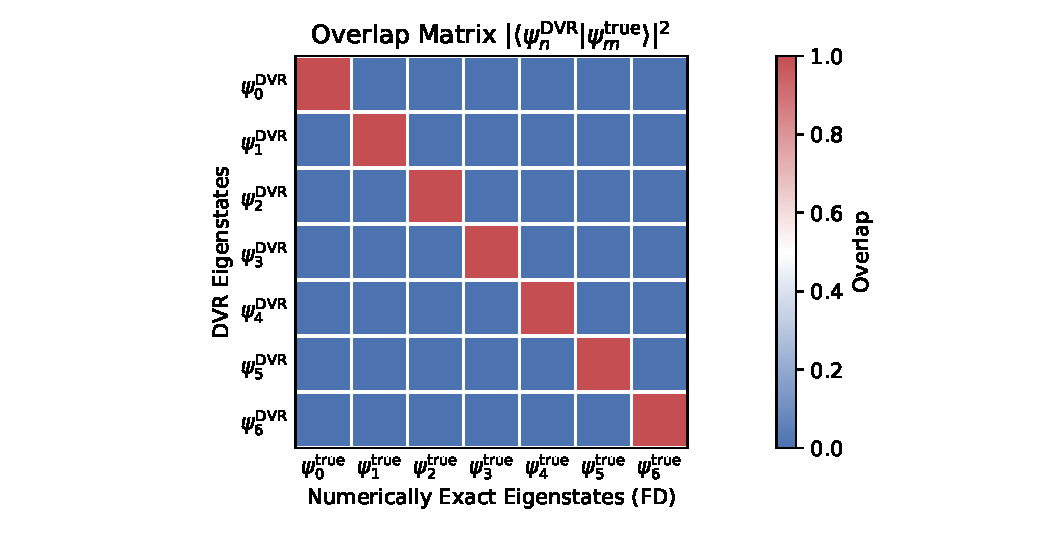
\includegraphics[width=\textwidth]{figs/dvr_validation_overlap.pdf}
    \caption{Overlap between the Sinc-DVR basis functions and the exact energy eigenstates of the Morse potential. The parameters used for the Morse potential are $D = 120.0$, $a = 1.0$, and $x_0 = 0.0$. The grid spacing is $\Delta x = 0.05$, and the number of grid points is $N = 600$ on a grid $x=[-1, 2]$.}
    \label{fig:dvr_validation_overlap}
\end{figure}
\\
Qualitatively, we see near perfect overlap between the Sinc-DVR basis functions and the exact energy eigenstates of the system. The diagonal elements of the overlap matrix exceed $0.9999$ for the 6 lowest lying states, indicating a fidelity of $99.99\%$ or higher, which is more than sufficient for our study. Due to the bound nature of the eigenstates in the Morse potential, we expect that the overlap should fall off rapidly when we are near the upper bounded state, and that is prevalent in the overlap matrix. Past eigenstate 7 (at $95.56\%$ overlap), the 8th and 9th eigenstate have an overlap of $73.86\%$ and $15.76\%$ respectively, the remaining states have an overlap below $10\%$. 
\subsubsection*{Energy spectrum}
Next, we compute the energy spectrum of the Morse potential using the Sinc-DVR basis and compare it to the exact energy eigenvalues. We follow the procedure outlined in section \ref{sec:sinc_dvr_validation}, and the resulting energies are shown in figure \ref{fig:dvr_validation}. The energy spectrum is shown in atomic units, and we see that the energy levels of the Sinc-DVR basis closely align with the exact energies of the system, especially for the lowest lying states—of which we are mostly interested in. 
\begin{figure}[h!]
    \centering
    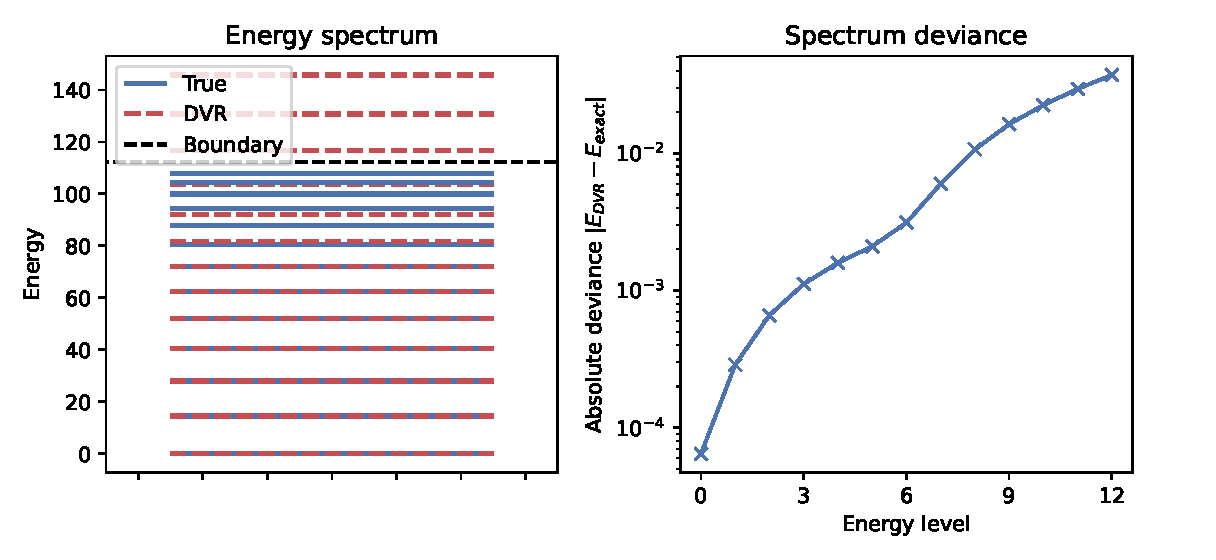
\includegraphics[width=\textwidth]{figs/dvr_validation.pdf}
    \caption{Comparison of the energy spectrum of the Morse potential using the Sinc-DVR basis and the exact energy eigenstates. The parameters used for the Morse potential are $D = 120.0$, $a = 1.0$, and $x_0 = 0.0$. The grid spacing is $\Delta x = 0.05$, and the number of grid points is $N = 600$ on a grid $x=[-1, 2]$. The energy spectrum of the lowest 13 eigenstates is shown in atomic units, blue line for the Sinc-DVR states and a red dashed line for the analytical eigenenergies. The absolute deviances is plotted logarithmically. The energy level of the upper bounded state is shown as a black dashed line.}
    \label{fig:dvr_validation}
\end{figure}

The DVR reproduces the ground-state energy exactly (within numerical tolerance), and the first four excited states to within $10^{-4}$ a.u. As seen in Figure \ref{fig:dvr_validation}, the absolute deviances of the energy eigenvalues are plotted logarithmically, and the first 8 eigenlevels have a relative error below $10^{-2}$. We see the clear limitation of the Sinc-DVR basis' ability to represent the higher order states, as their energies move above the bounded spectrum of the Morse potential trap. Furthermore, we see also how the energy deviation increases rapidly when moving towards the bounded states where the analytical solution 'squeezes' the energy levels together. The Sinc-DVR basis is not able to capture this 'squeezing' effect, and thus, the energy deviation increases as we move towards the boundary. 
As we are mostly interested in the lowest lying states, we do not mind the increasing error for the higher order states, or the lack of 'squeezing', as these levels are not directly relevant for our quantum control protocols, outside of the possibility to alter the dynamics of lower lying states should there occur population leakage to these higher-order states near the boundary.
\subsubsection{Implications and convergence}
Taken together, the near-perfect overlaps and sub-Hartree energy errors demonstrate that the Sinc-DVR basis introduce negligible residual errors in the representation of the energy eigenstates and the energy spectrum of interest in the Morse potential. If we desire, we may further reduce the error by increasing the number of grid points $N$ (or decreasing the grid spacing $\Delta x$). We therefore proceed with confidence that the Sinc-DVR basis is a suitable choice for our quantum control protocols, as it accurately captures the essential relevant features of the system. The grid spacing used here is much finer than what we aim for in the study of the double-well Morse potential. Most important for us is that the low-lying states in the system are well-represented as they are the targets for our quantum control protocols. 

Setting up a test scenario with the following parameters $D = 60.0, a = 0.4$, we find that the Sinc-DVR basis with $N=30$ grid-points on a grid $x = [-5, 10]$ with a grid spacing of $\Delta x = 0.5$ a.u. yields an overlap of $>99.00\%$ for the first 4 eigenstates. This indicates that it is not only the grid spacing that matters, but also the distance from the boundary of the grid. The Sinc-DVR basis accurately captures the low-lying states but fail to properly 'squeeze' the higher-order states when we approach the upper bound of the potential trap. For this reason, we will use a larger grid spacing of $\Delta x = 0.5$ a.u. in the study of the double-well Morse potential, while making certain that the states we are interested in are well below the uppe bound $l \leq \sqrt{2D}/a$, which is approximately $l \leq 27$ for the potential used in this test scenario. With this information at hand, it is imperative that we then construct our potential to be deep enough that the relevant states we wish to investigate lie far away from the boundary of the potential trap.


\subsection{Numerical propagator benchmarks}
To systematically validate our implementation of the aforementioned numerical methods (Section \ref{sec:time_evolve_methods}), we require a simple yet representative quantum system that exhibits non-trivial dynamics but still has closed form solutions for comparison. For this purpose, we will once again turn to the simple Landau-Zener model \eqref{eq:landau_zener}, introduced in Section \ref{sec:avoided_crossings}. This simple two-level system is governed by a time-dependent Hamiltonian. It captures the essential features of quantum dynamics, making it an ideal testbed for our numerical methods in preparation for the more complex double-well Morse potential system we shall study.
Recall, the Hamiltonian for the Landau-Zener model is given by:
\begin{align*}
    H(t) = \begin{pmatrix}
        vt & V \\
        V & -vt
\end{pmatrix},
\end{align*}
where $v$ is the sweeping velocity, $V$ is the coupling strength, and $t$ is the time. At $t=0$, the uncoupled system would have a degeneracy, but the coupling $V$ opens a gap (lifts the degeneracy), resulting in an avoided crossing as we saw in section \ref{sec:avoided_crossings}. Thus, this minimal system captures one of the simplest non-trivial dynamics of a quantum system, which also allows for closed form solution for the transition probability \eqref{eq:landau_zener_trans_prob}. 

This makes an excellent textbed for our numerical integrators due to the following reasons:
\begin{itemize}
    \item \textbf{Low dimensionality:} The Landau-Zener model is a two-level system, making it computationally efficient to simulate and analyze. This allows us to focus on the numerical methods without being overwhelmed by the computational complexity of the system.
    \item \textbf{Non-trivial dynamics:} The system exhibits interesting dynamics, such as transitions between states, which require the numerical implementations to accurately capture the time evolution of the wavefunction. This provides a meaningful test for the accuracy and stability of the numerical methods.
    \item \textbf{Analytical reference:} The Landau-Zener model has well-known analytical solutions for the transition probabilities and wavefunction dynamics, allowing us to directly compare the results of our numerical methods against these exact solutions. This serves as a benchmark for assessing the performance of the numerical methods.
\end{itemize}
\subsubsection*{Benchmark procedure}
We initialize the system in the lowest lying state $\ket{\Psi(0)} = (1, 0)^T$, which corresponds to the ground state of the uncoupled system, from an initial time $t_0<0$ to a final time $t_f>0$. We will then compare:
\begin{itemize}
    \item Global error vs. simulation time $T$: How the methods converge towards the closed form solution.
    \item Runtime efficiency: How fast each method can compute the transition probability.
    \item Stability during evolution: How well each method handles long time simulations. 
\end{itemize}
\\ 
We numerically propagate an initial wavefunction prepared in the ground state of the uncoupled system, and compute the final transition probability $P_{12}$, given analytically by \eqref{eq:landau_zener_trans_prob}. In other words, after the sweep we compute 
\begin{align*}
    P_{1\to2} = |\braket{\Psi_2|\Psi(t_f)}|^2,
\end{align*}
the probability of finding the system in the excited state $\ket{\Psi_2}$ at time $t_f$, given that it was initially prepared in the ground state $\ket{\Psi_1}$. The Landau-Zener transition probability is derived in the infinite time-limit, i.e $t\rightarrow \pm \infty$, so this analysis illustrate how each numerical method converges to the analytical solution as total simulation time increase.
\begin{figure}[h!]
\centering
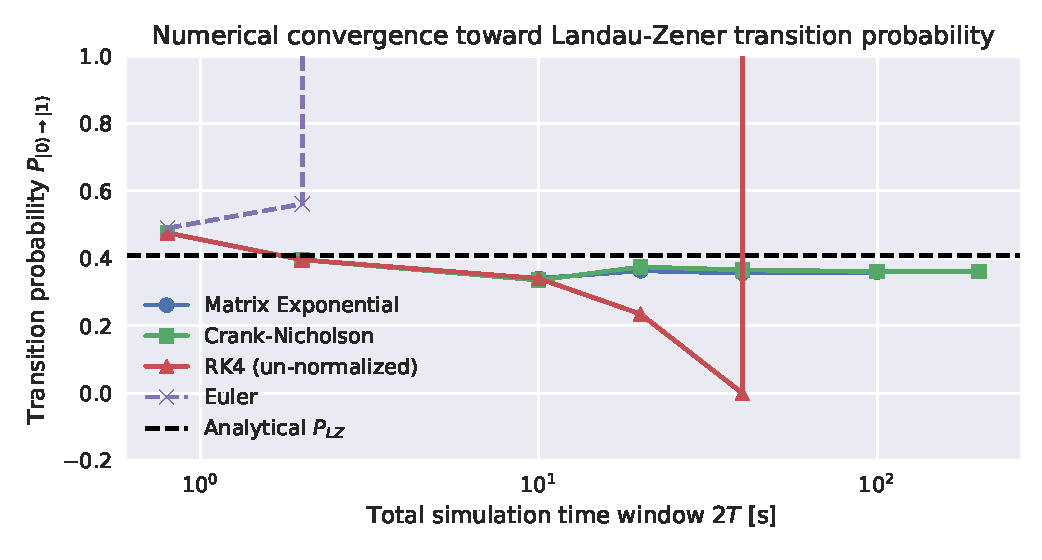
\includegraphics[width=1.0\textwidth]{figs/landau_zener_convergence_benchmark.pdf}
\caption{Final transition probability using $v=7.0$, $V=1.0$, computed with various numerical methods for increasing total simulation time $
2T$. We see that Crank-Nicolson and matrix exponentiation converge towards the analytical Landau-Zener probability (dashed line), with RK4 showing good accuracy until instability sets in at longer times due to lack of normalization. The x-axis is in logarithmic scale.}
\label{fig:landau_zener_convergence_benchmark}
\end{figure}

As we can see in figure \eqref{fig:landau_zener_convergence_benchmark}, some of the methods converge towards the analytical solution within certain timeframes, with varying degrees of stability. The Euler method diverges rapidly, as expected, due to its explicit nature and lack of normalization corrections. The more robust RK4 method remain stable and follow closely with the more sophisticated methods, before the accumulated error in the norm blows it up. Both of these methods can be improved upon by introducing norm corrections, at a computational cost (albeit minimal). The Crank-Nicolson method, on the other hand, remains stable and accurate for longer simulation times, as it preserves unitarity by construction. We also see that every method undershoots the analytical probability by a few percentages, and we expect this deviance to dissapear completely for even longer timespans. The reason for this is due to the asymptotic nature of the analytical expression, and how well the initial state accurately models the "true" ground state. At $t_{0} = -T/2$, for a finite $T$, the off-diagonal terms are non-zero giving rise to \emph{minor} mixing which will vanish as $T$ is increased. The culmination of both of these errors are seen as the deviance between "true" transition probability $P_{LZ}$ and the numerically computed probabilites. 
\\ 

To assess the computational speed of the numerical methods, a full Landau-Zener simulation was measured using the \texttt{time.perf\_counter()} function in Python, which provides a high-resolution timer suitable for short time measurements.This measurement also includes system overhead, yielding realistic performance metrics to evaluate each method. 
The benchmark was performed for the two-level system with sweeping parameter $v=7.0$, coupling strength $V=1.0$, and a time integration interval of $t \in [-5, 5]$ with $100{,}000$ time steps, i.e a time-step of $\Delta t = 10^{-4}$s. The results are presented in the following table \eqref{tab:landau_zener_runtime}, along with remarks on their performance characteristics.

\begin{table}[h!]
\centering
\caption{Runtime comparison of time propagation methods for the Landau-Zener model ($v = 7.0$, $\Delta = 1.0$, $t \in [-5, 5]$, 100,000 steps). Timing measured using \texttt{time.perf\_counter()}.}
\begin{tabular}{l c l}
\toprule
\textbf{Method} & \textbf{Time (ms)} & \textbf{Remarks} \\
\midrule
Matrix Exponential & 5942.1 & Most accurate, but very slow \\
Euler              & 828.6  & Fastest, but unstable \\
RK4                & 2621.0 & Balanced performance \\
Crank--Nicholson   & 1953.6 & Stable and efficient \\
\bottomrule
\end{tabular}\label{tab:landau_zener_runtime}
\end{table}
The table \eqref{tab:landau_zener_runtime} shows that the matrix exponential method is the slowest, but also it is exact, while the Euler method is the fastest but unstable and inaccurate for longer simulations. The RK4 method is a good compromise between speed and accuracy, while the Crank-Nicolson method is stable and efficient, and—in our novel unoptimized implementation— outperforms the speed of RK4. This is generally not the case however, as for most system of moderate size, the linear system of equations in CN is more expensive to solve than the matrix products in RK4. 

In conclusion, the convergence plot together with the runtime analysis shows that the Crank-Nicolson method is the most suitable for long time simulations, as it preserves unitarity and stability, for cases where direct matrix exponentiation is not feasible. We have confirmed that the explicit Taylor-expansion methods (Euler and RK4) can work over shorter intervals, but they require norm corrections, and small time steps to remain reliable for longer simulations. Direct matrix exponentiation is unbeatable with regards to accuracy, but scales exponentially in computational cost. Crank-Nicolson hits a sweet spot: It is unconditionally stable, preserves unitarity, and is computationally efficient for long time simulations. 

Because our goal is to simulate two interacting particles trapped in a double-well potential, in a Hartree-reduced basis, we choose to employ direct matrix exponentiation whenever possible, and to default Crank-Nicolson for extended time-simulations. While one could explore more advanced methods, we firmly believe that the Crank-Nicolson method is sufficient for our purposes, as it provides a good balance between accuracy, efficiency and simplicity.
\end{document}